\section{The Weekplanner Application}

The focus in both this semester and last year on the GIRAF project was on the Weekplanner application. The following section describes the application.

\subsection{Purpose}
Many people with autism need structure. It is important to find a way to communicate what they should expect during the day. This can prove challenging, especially when they are placed high on the autism spectrum, or have limited verbal communication.\\
One way to communicate, that is often used, is with visual support\cite{VisualSupport}. There is a broad range of ways to do this. One way is with the help of pictures. Each picure represents an activity.

\begin{figure}[H]
    \begin{center}
        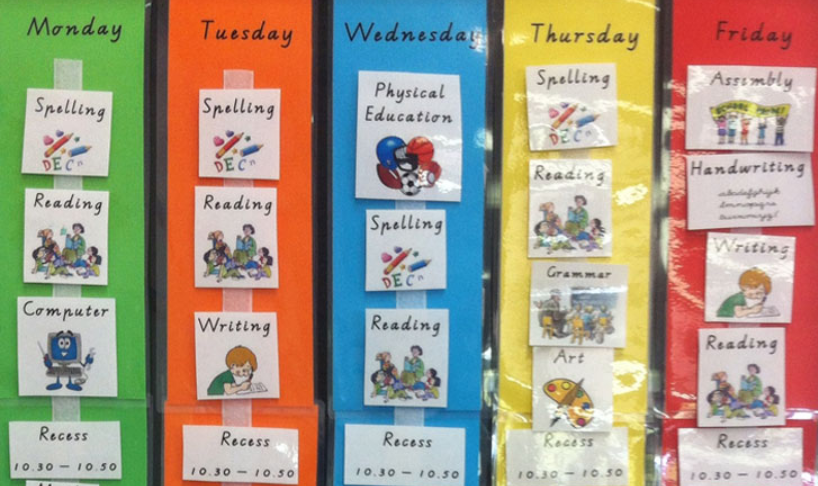
\includegraphics[width=0.95\textwidth]{figures/WeekPlanEks.png}
    \end{center}
    \caption{An example of a weekplan.\cite{VisualSupport}}
    \label{fig:WeekPlan}
\end{figure}

As seen on \autoref{fig:WeekPlan}, the activities can be structured in days. Each day has a series of activities, and each activitie is represented by a picture.\\
Though this is a common method of structuring activities, it has some problems. First of all, it is unflexible. It can not be carried around and the amount of activities can't exceed the size of the board. Second, it is difficult to add new pictures and insert one. 
Therefore, many institutes want a digital version of this, which is why the GIRAF project build the Weekplanner application.\\

\subsection{Features}
There are two types of users, guardian and citizen. The weekplans are connected to a citizen, but they cannot log into the system themselfs. Guardians can log into the system, and get a list of citizens they are working with. When they choose a citizen, all the weekplans that citizen has are shown.\\
Here the guardian can edit the weekplan, or change to citizen mode. In citizen mode, the different activities can be marked as done, but a citizen cannot change the weekplan or navigate the application. From citizen mode, the system can be changed back to guardian mode.\\
The following describes only the screens that was implemented in the beginning of the semester. When this section was written, we had shifted the framework of the application\ref{sec:MovingTheFrontend}. We also moved the servers to another location.\\
This ment that the application on Google Play could not login. It was not possible to build the application later, so we could not get pictures of the actual application. The pictures in this section is from the prototypes made by \gls{POT}.\\ 

The screens are:
\begin{itemize}
    \item Login
    \item Select citizen 
    \item Select Weekplan 
    \item Weekplan
    \item Find Pictogram
\end{itemize}

Here follows descriptions of each screen. The pictures are prototypes made for the costumers by \gls{POT}. 

\subsubsection*{Login Screen}
The login screen is similar to a standard login screen. The prototype can be seen in \ref{fig:LoginProt}

\begin{figure}[H]
    \begin{center}
        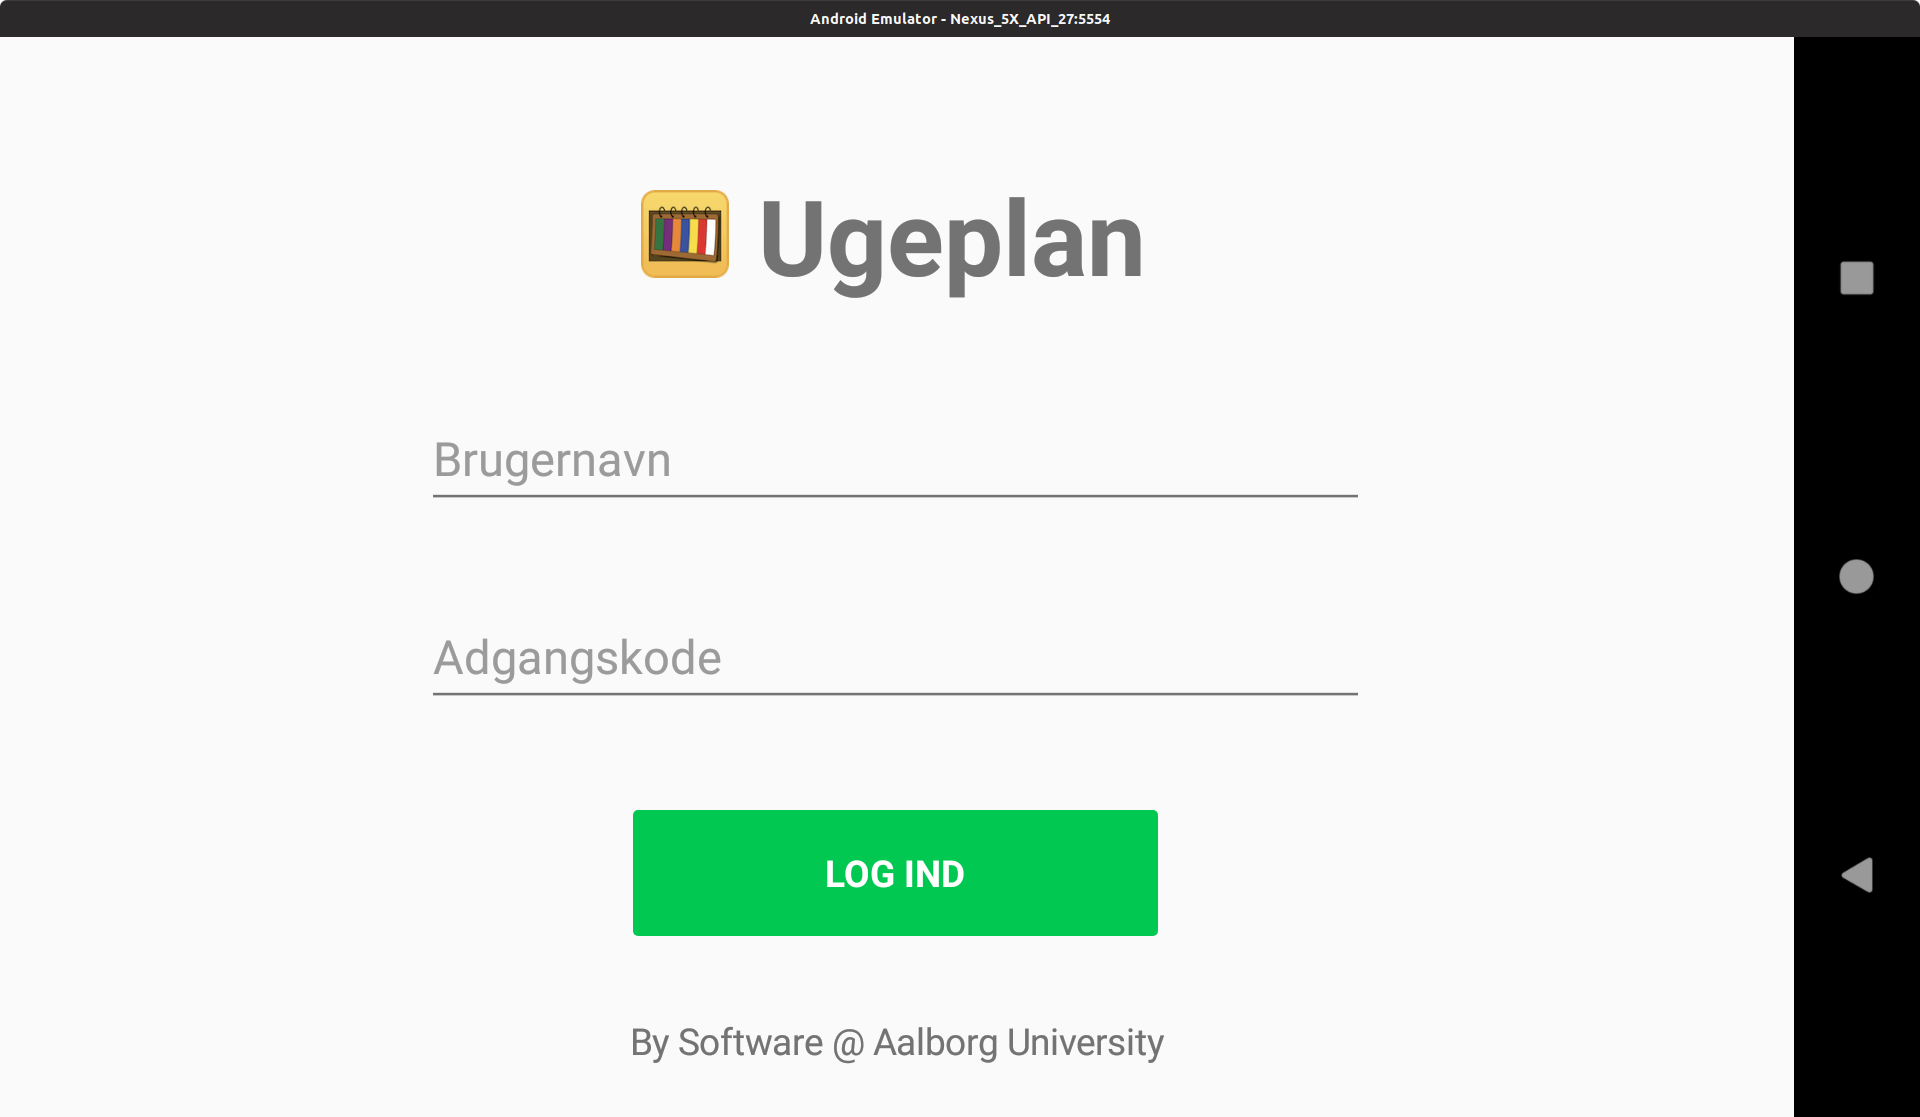
\includegraphics[width=0.95\textwidth]{figures/Prototypes/LoginScreenPrototype.png}
    \end{center}
    \caption{The prototype for the login screen}
    \label{fig:LoginProt}
\end{figure}
The application navigates to the Select Citizen screen after login. 

\subsubsection*{Select citizen screen}
The select citizen screen is shown in \ref{fig:ChooseCitProt}

\begin{figure}[H]
    \begin{center}
        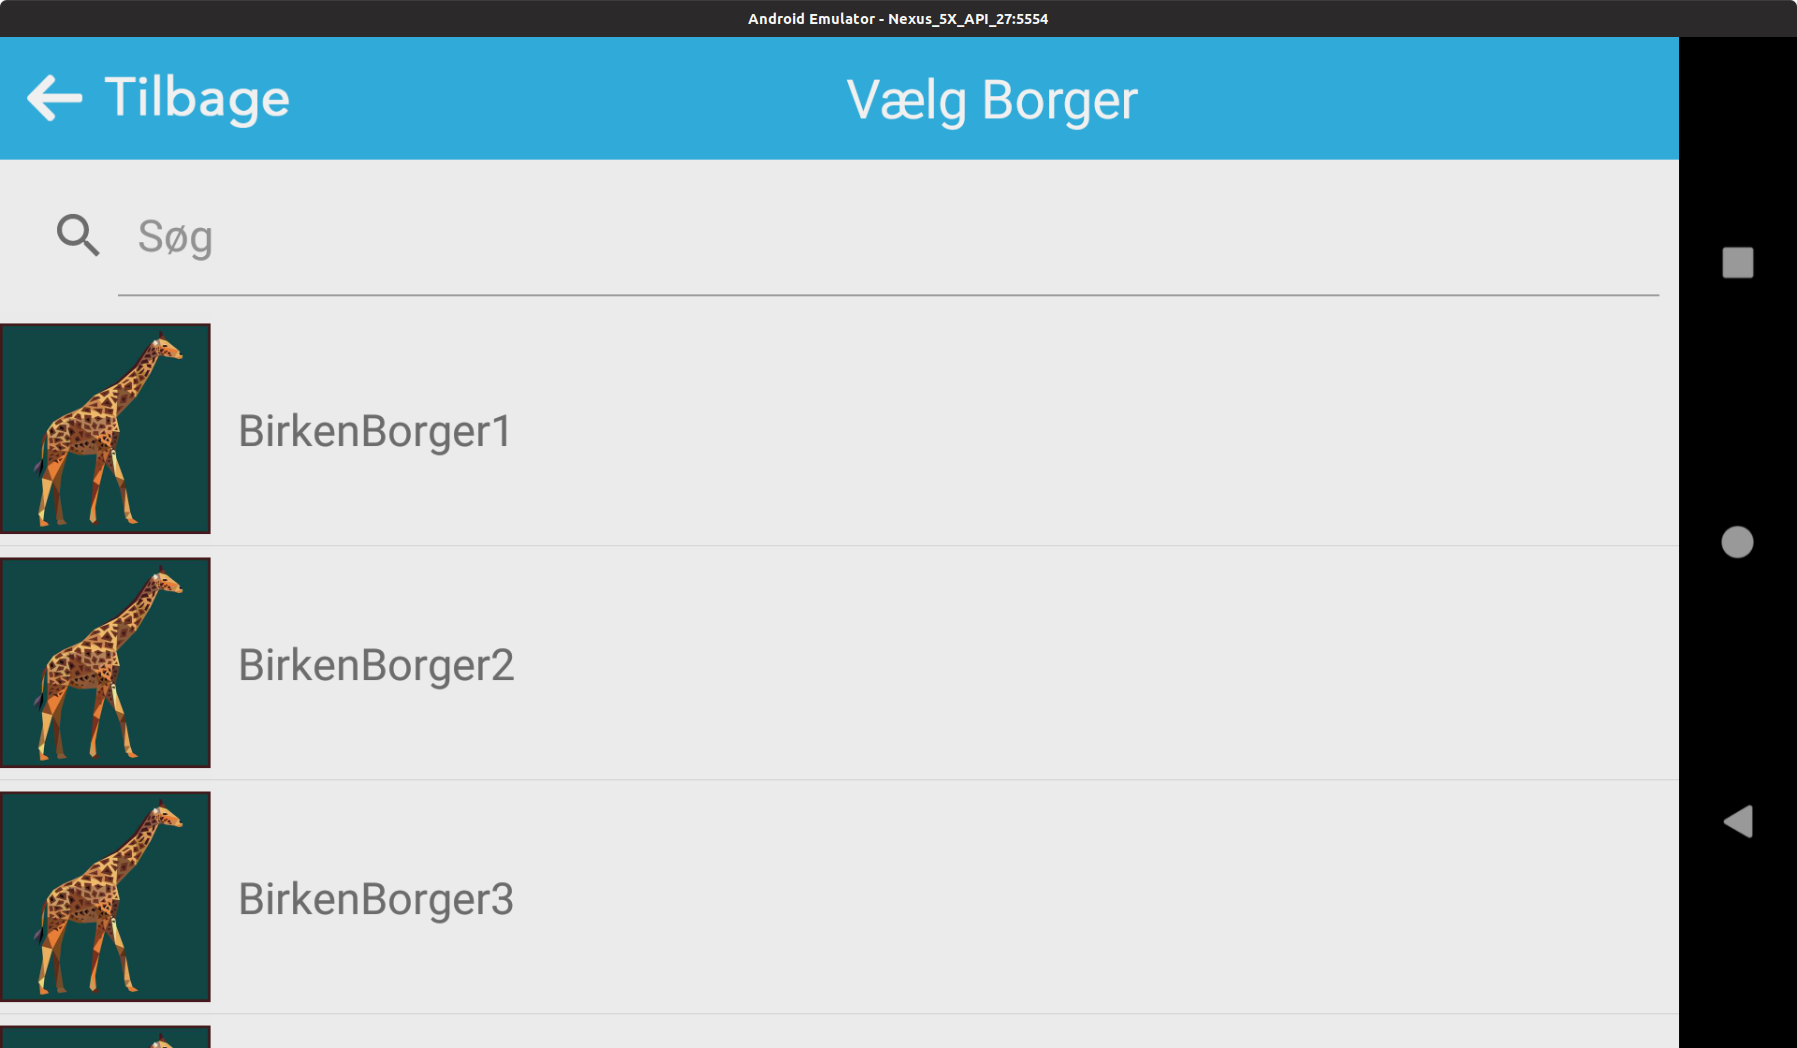
\includegraphics[width=0.95\textwidth]{figures/Prototypes/ChooseCitizenPrototype.png}
    \end{center}
    \caption{The prototype for the select citizen screen}
    \label{fig:ChooseCitProt}
\end{figure}

Here the guardian get a list of every citizen connected to him. The guardian can click on a citizen and then be directed to the Select Weekplan screen. 

\subsection*{Select Weekplan Screen}

\ref{fig:ChooseWeekProt} shows how the choose weekplan screen should look.
\begin{figure}[H]
    \begin{center}
        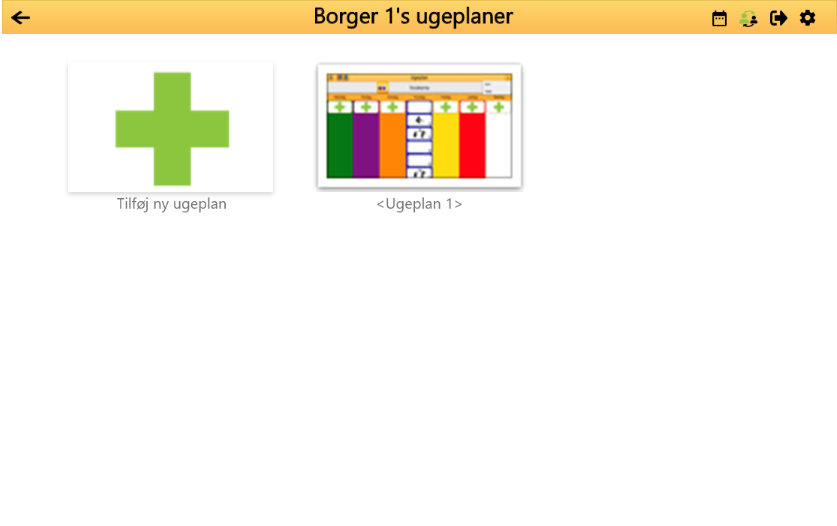
\includegraphics[width=0.95\textwidth]{figures/Prototypes/SelectWeekplanPrototype.png}
    \end{center}
    \caption{The prototype for the select weekplan screen}
    \label{fig:ChooseWeekProt}
\end{figure}

For each weekplan connected to the choosen citizen, a picture of the weekplan with it's name is shown. There is also a button for adding a new weekplan to the citizen.\\
The guardian is directed to the weekplan screen after choosing a plan.\\

\subsection*{Weekplan Screen}
There are two types of weekplan screens, the citizen screen, \ref{fig:WeekplanCitProt}, and the guardian screen, \ref{fig:WeekplanGuarProt}. 

%De to kunne måske være side om side??
\begin{figure}[H]
    \begin{center}
        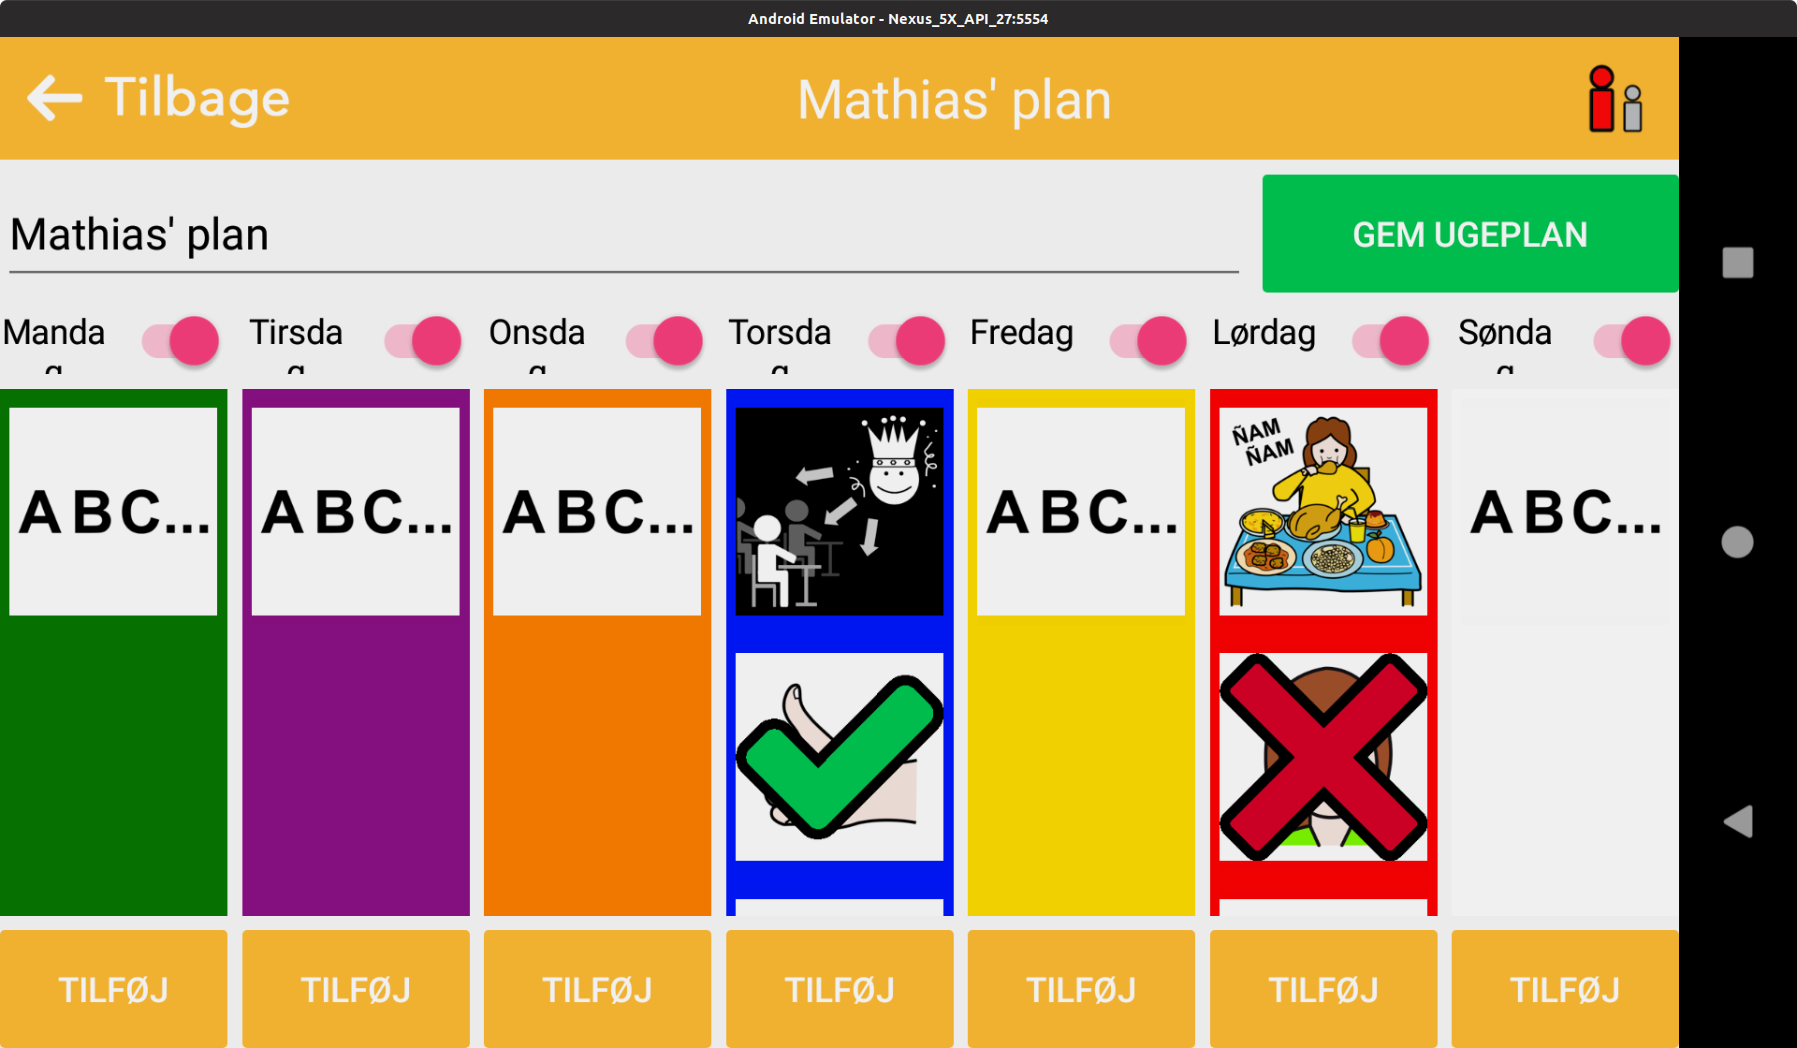
\includegraphics[width=0.95\textwidth]{figures/Prototypes/WeekPlannerGuardianPrototype.png}
    \end{center}
    \caption{The guardian version of the weekplan screen}
    \label{fig:WeekplanGuarProt}
\end{figure}

\begin{figure}[H]
    \begin{center}
        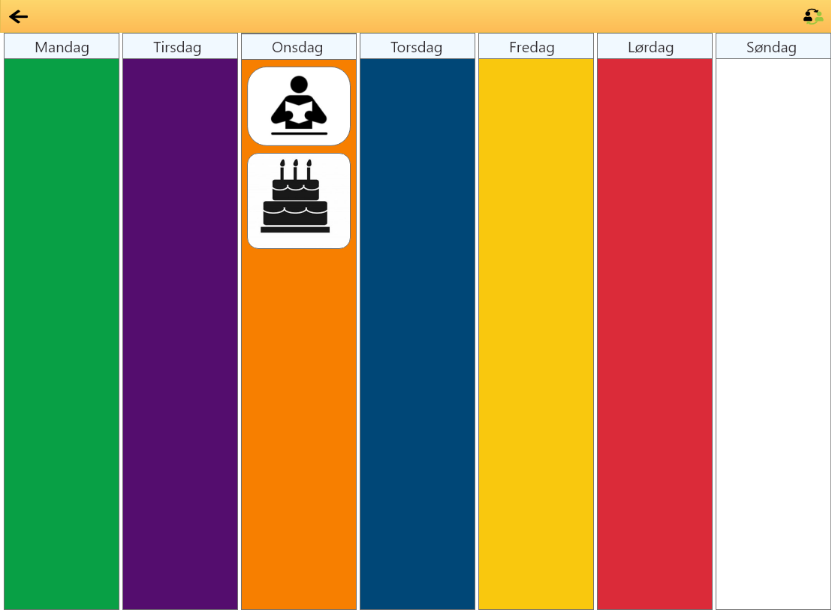
\includegraphics[width=0.95\textwidth]{figures/Prototypes/WeekPlannerCitizenPrototype.png}
    \end{center}
    \caption{The citizen version of the weekplan screen}
    \label{fig:WeekplanCitProt}
\end{figure}

In both screens you can see the activities planned for the day, but when an activities is clicked on, on the citizen screen, they are marked as done, while they can be edited on the guardian screen. The guardian screen is also the only screen where you can add activities.

The features working on the start of the semester is the following:
\begin{itemize}
    \item Login 
    \item Choose citizen 
    \item Choose weekplan
    \item Mark activity as done 
    \item Add activity
    \item Remove activity
    \item Switch to guardian mode
\end{itemize}

The features are the basic features of the application. Some other features are planned in the future. 
